\section{Background}
\label{sec:background}

\subsection{Physical samples}

The physical samples are prepared for SR$\mu$CT scanning by cutting out a portion from a larger
12mm cylindrical sample. \aleksandar{Why? We should include a brief chronological tour of how the
sample has been handled from before until now?} The cut samples are cubes of size
(6.478mm, 6.478mm, 6.146mm) in the x,y,z direction respectively. This contains the titanium dental
implant (Astra Tech OsseoSpeed, ST Molndal, Sweden), which is 3.5mm in diameter and 8mm long. Along
its length the lower 5.5mm has larger threads and is attached to recipient bone. The upper 2.5mm
has smaller threads and is where newly formed bone is to be assessed. Sorrounding the bone and
implant contact-region are cavities containing resin, air, blood vessels and other fibrous tissue.

\begin{figure}
\centering
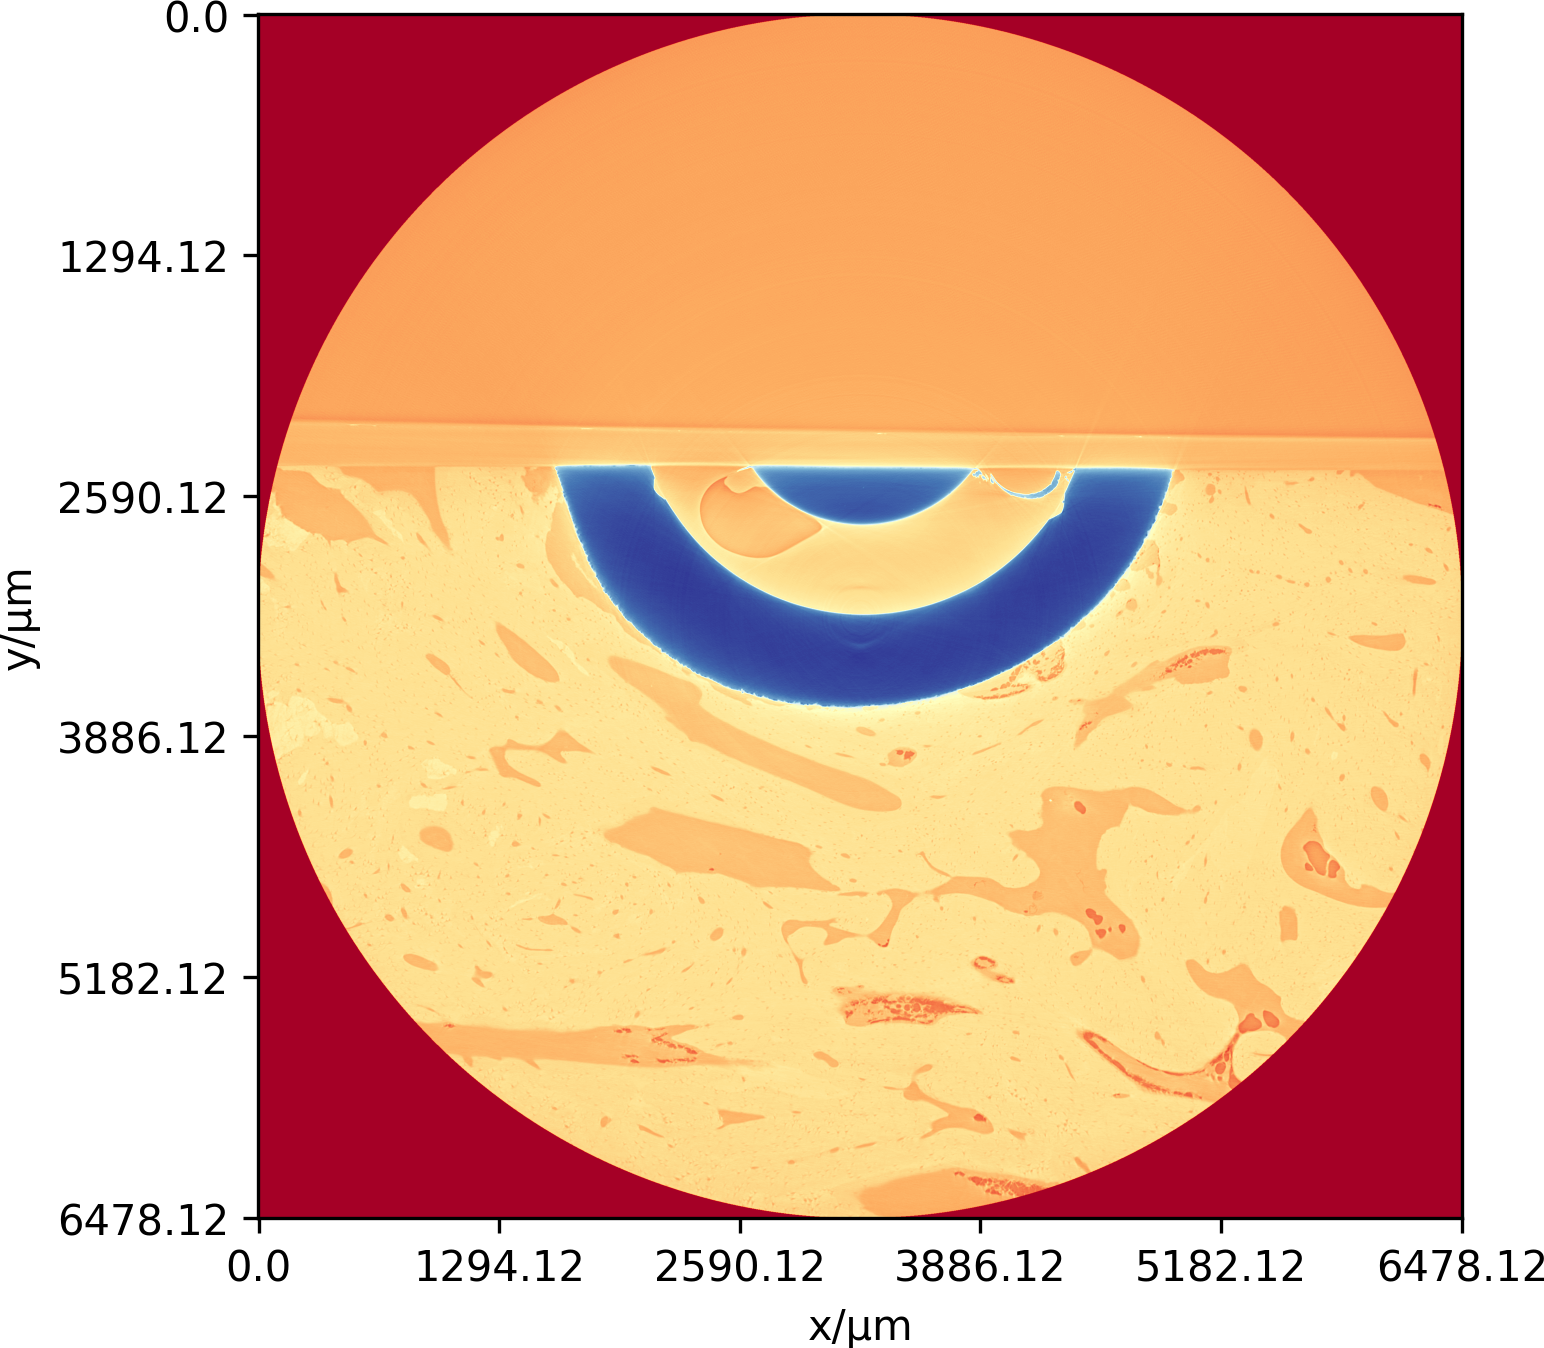
\includegraphics[width=0.96\columnwidth]{figures/770c_pag-full-xy-1x.png}
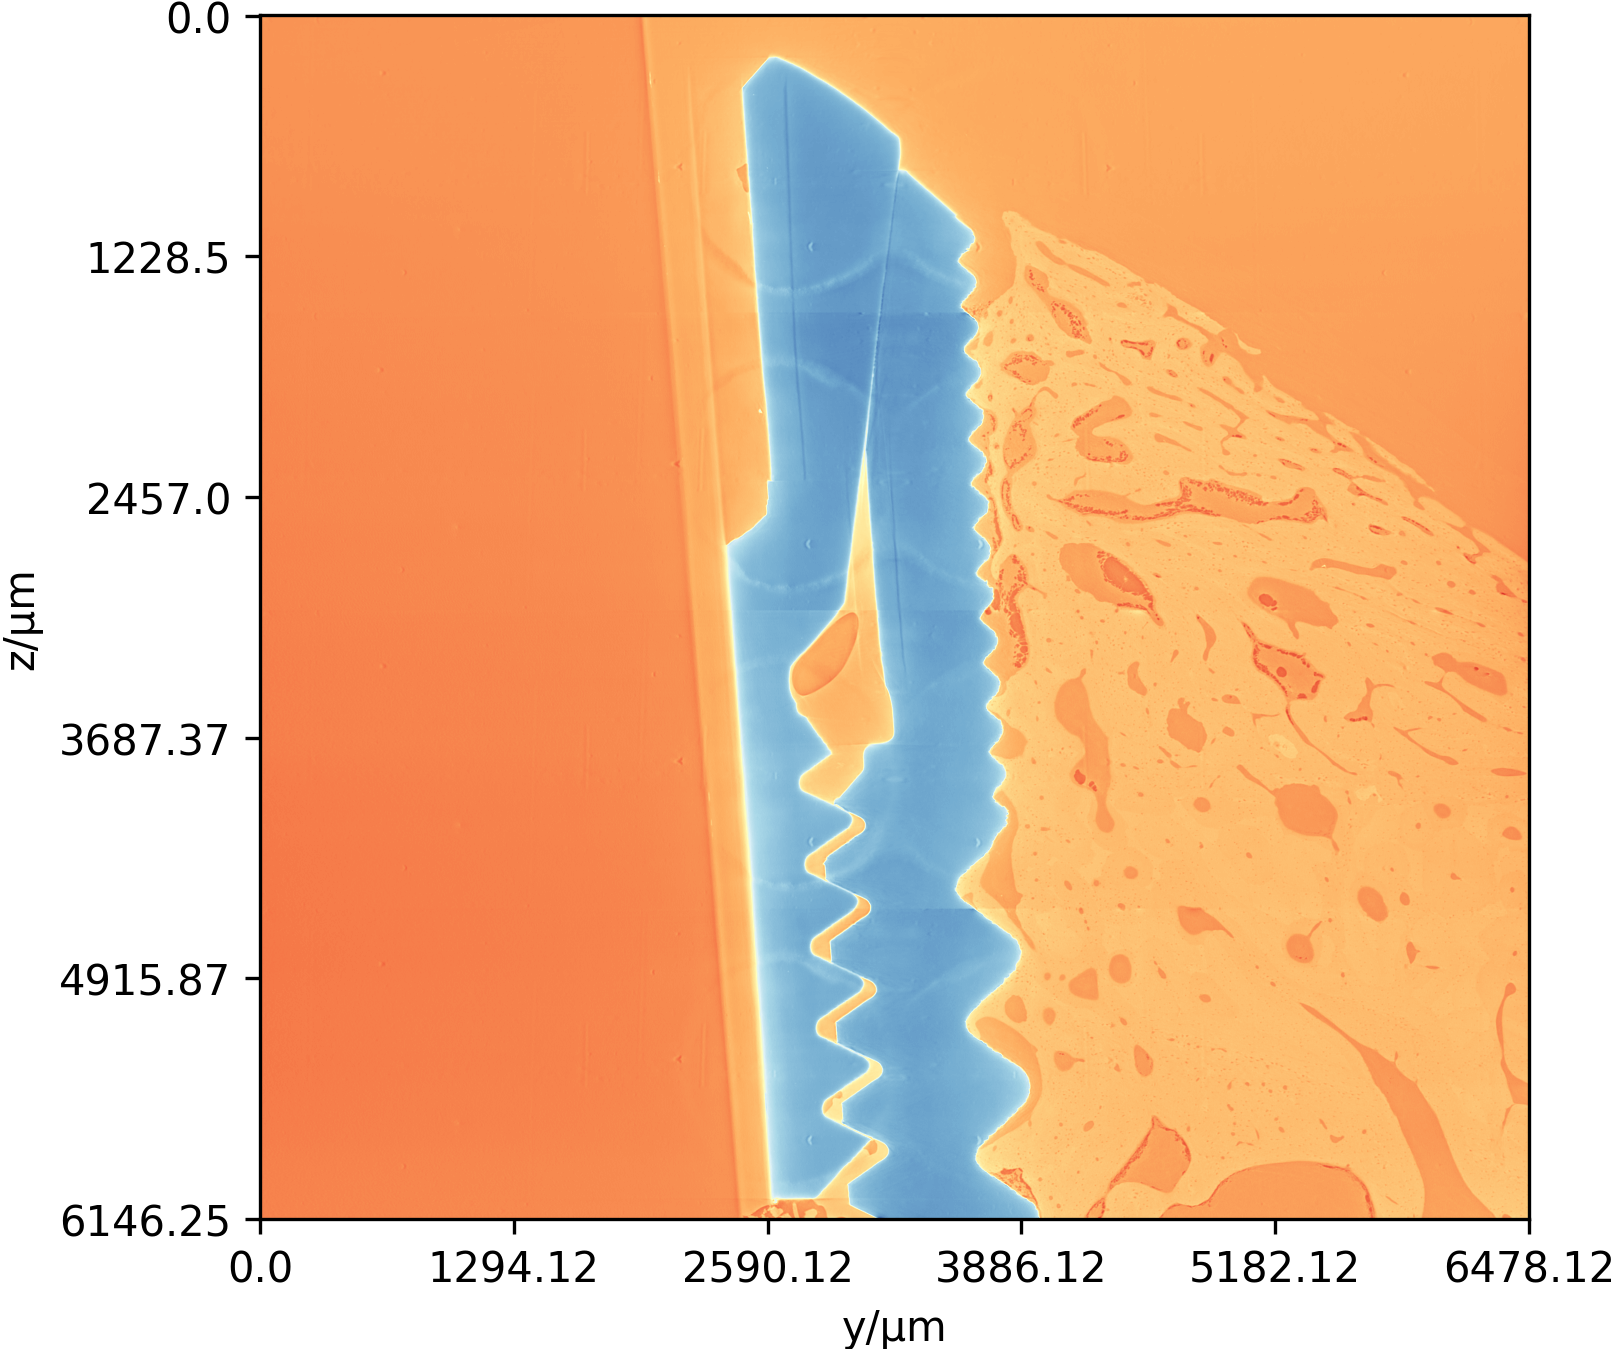
\includegraphics[width=0.96\columnwidth]{figures/770c_pag-full-yz-1x.png}
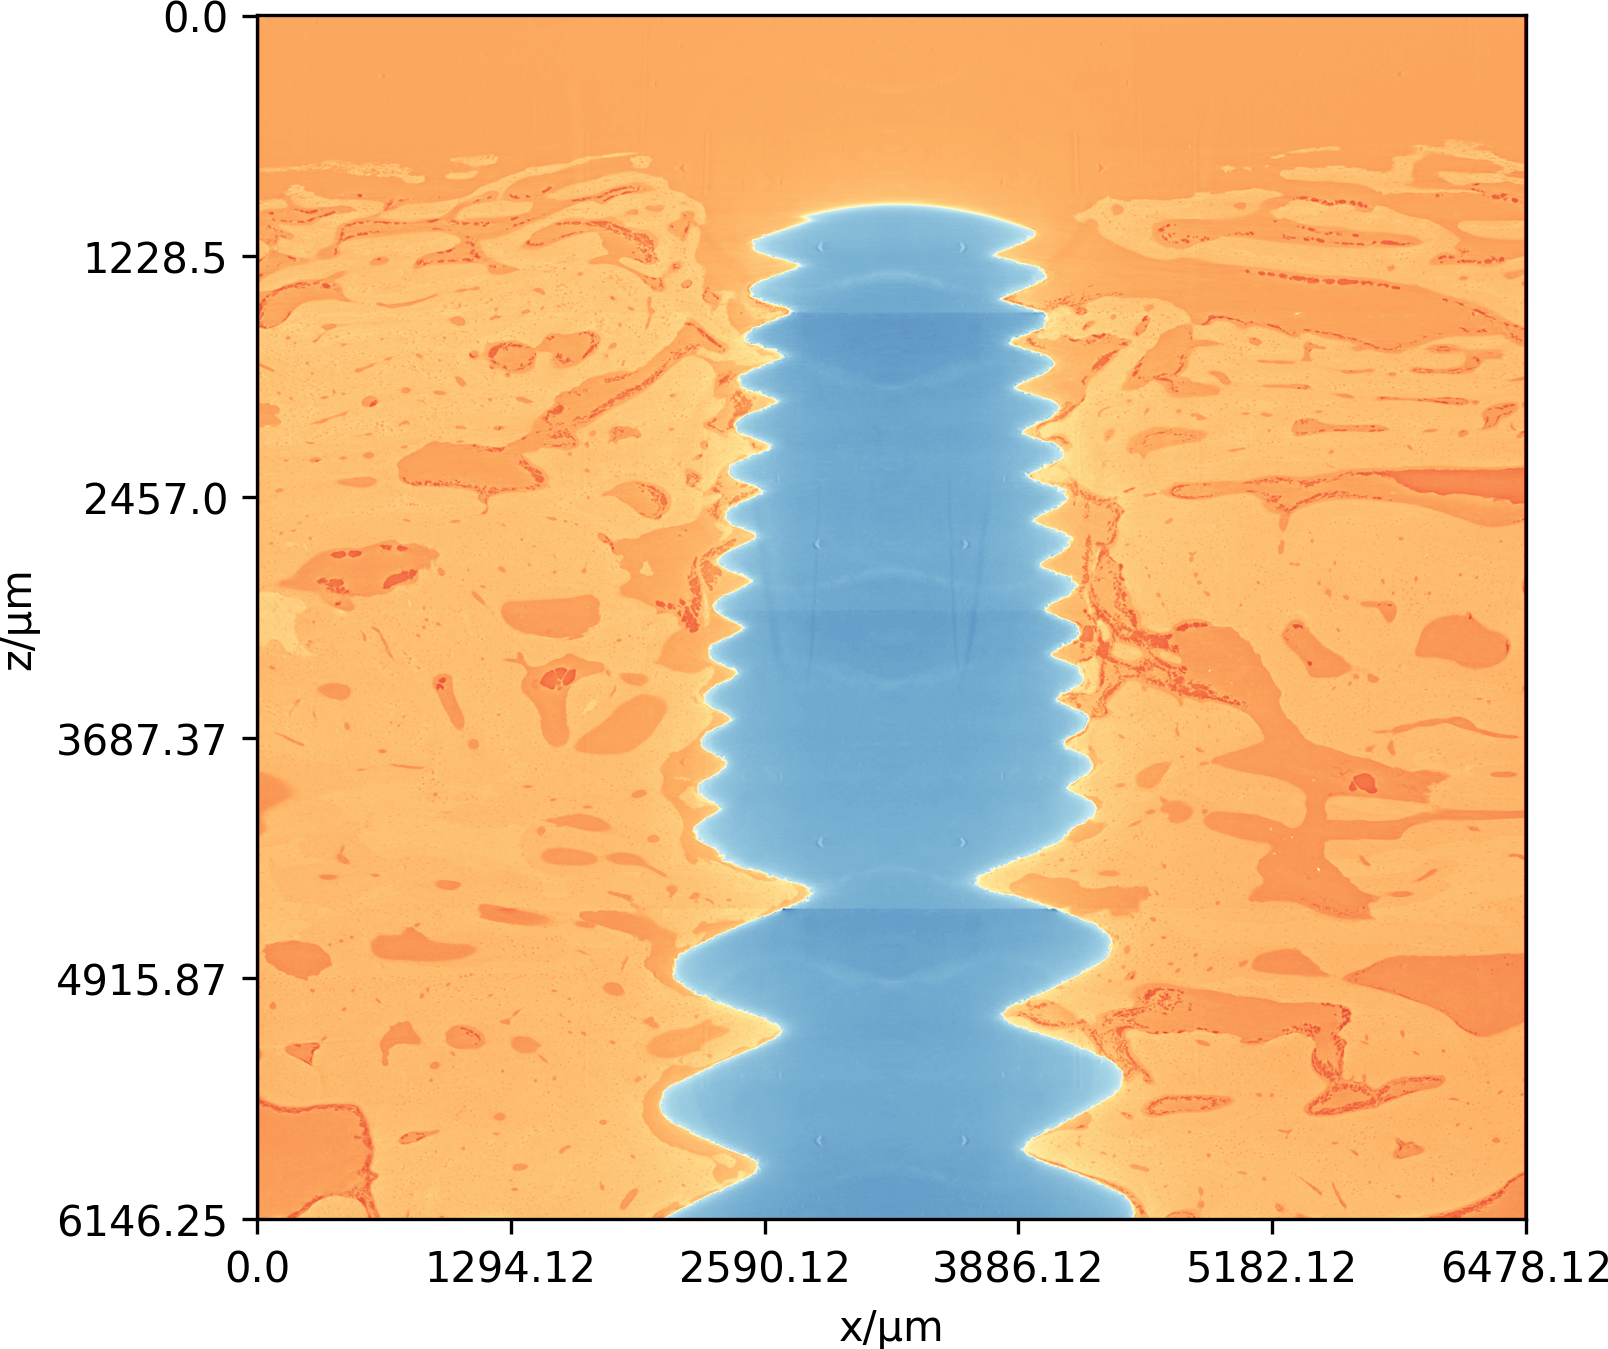
\includegraphics[width=0.96\columnwidth]{figures/770c_pag-full-xz-1x.png}
\caption{Full sample seen as cross sections in XY, YZ, XZ planes respectively. A voxel has size of
1.875$\mu$m. Red voxels are numerically low, while blue are high.}
\label{fig:3viewsample}
\end{figure}

This is shown in three different cross sectional views
in \cref{fig:3viewsample}. Each material has a unique density and thus absorption. The titanium
implant shown in blue has higher absorption than bone. Bone material shown in light orange has
higher absorption than its sorrounding dark orange colored regions containing blood vessels
tissue, air and resin.

\subsection{Data acquisition}

It can be difficult to study and evaluate the bone structure and blood network without destroying
or manipulating the sample. X-ray computed tomography is a widely used tool for non-intrusive medical
imaging. By exposing a subject to X-rays, we can map the linear attentuation coffecient of the passing
rays. Each ray is attenuated relatively to the density and composition of the material it passes.
By rotating either the scanner or the sample we can get a full 3D image representation of the inner
structure of the sample. Each volumetric pixel (voxel) then represents the X-ray attenuation at its
spatial position. We can therefore reliably use X-rays to internally characterise samples in a
non-intrusive and non-destructive manner. Medical CT-scans can provide spatial resolutions on the
order of submillimetre scale \citep{medicalct}. The more modern micro computed tomography ($\mu$CT)
can provide much higher spatial resolution on the micrometre scale \citep{srexptime}.

This work focuses on data acquired by Synchrotron Radiation micro-CT (SR$\mu$CT). For this imaging
technique, electrons are accelerated to ultra-relativistic speeds in trajectories directed by strong
magnetic fields. Contrary to both CT and $\mu$CT, this approach requires a large particle accelerator,
and is not standard medical or laboratory equipment. The added complexity means that SR$\mu$CT can
offer an even better spatial resolution of up to 0.1 $\mu$m. The resulting beams are high in
brilliance and collimation which gives a very clear signal. Its mono-energetic nature also means
that images are not subject to artifacts from beam-hardening.
\carl{\textbackslash label\{initial-beam-claim\}}
The data presented here has been
acquired at the ID19 beam line at the European Synchrotron Radiation Facility (ESRF) in Grenoble,
France, and has previously \aleksandar{ref to former article} been reconstructed using the Python
framework PyHST \citep{pyhst}.

\subsection{Image data}

Each image sample contains voxels with a spatial resolution 1.875$\mu$m. The full physical size of
a sample is about 6.5mm, which makes the raw dimensions of a single image $(3480,3480,3384)$ pixels.
For computational purposes, this has been cropped to be divisible by a power $2^N$ or more
specifically $2^5=32$ in our case. A full image sample is further split into 4-6 sub-volumes through
the height of the implant. This gives a size of $(3456,3456,810)$ pixels per sub-volume, where the
last axis gets stacked for a full volume. \aleksandar{OBS: 846 i rå størelse, 810 er efter
volume-matching. -- Should ideally also explain a bit about how the samples were cut during
acquisition. How were the samples secured in order not to be physically shifted too much etc.}

\subsection{Physical effects, noise and artifacts}
\label{sec:physics}

Noise in tomography is unavoidable, and it makes segmentation harder because it further obscures
the boundaries between materials. Matarials may be well separated from certain angles in the
3d-reconstructed image, but overlap from others. Some noise like that corrected by flat-field
correction is very uniformly distributed across images. Some noise is however very spatially
dependent on its sorrounding regions. Knowing the composition and positioning of the materials
being imaged, we can counter some of these effects during segmentation. The noise effects manifest
themselves as numerical shifts in voxel-values as a function of their position. This is a direct
result of a misrepresented attenuation along the axis the X-rays are passing.

This orientation dependency illustrates how voxel intensity values are not globally fixed. How a
certain material is represented in intensity, is highly dependent on its position relative to
neighbouring regions. Especially since this also determines the amount and type of derived noise. 
The same material with the same density, can thus be represented at multiple varying intensities
within the same sample.

\begin{figure*}
\centering
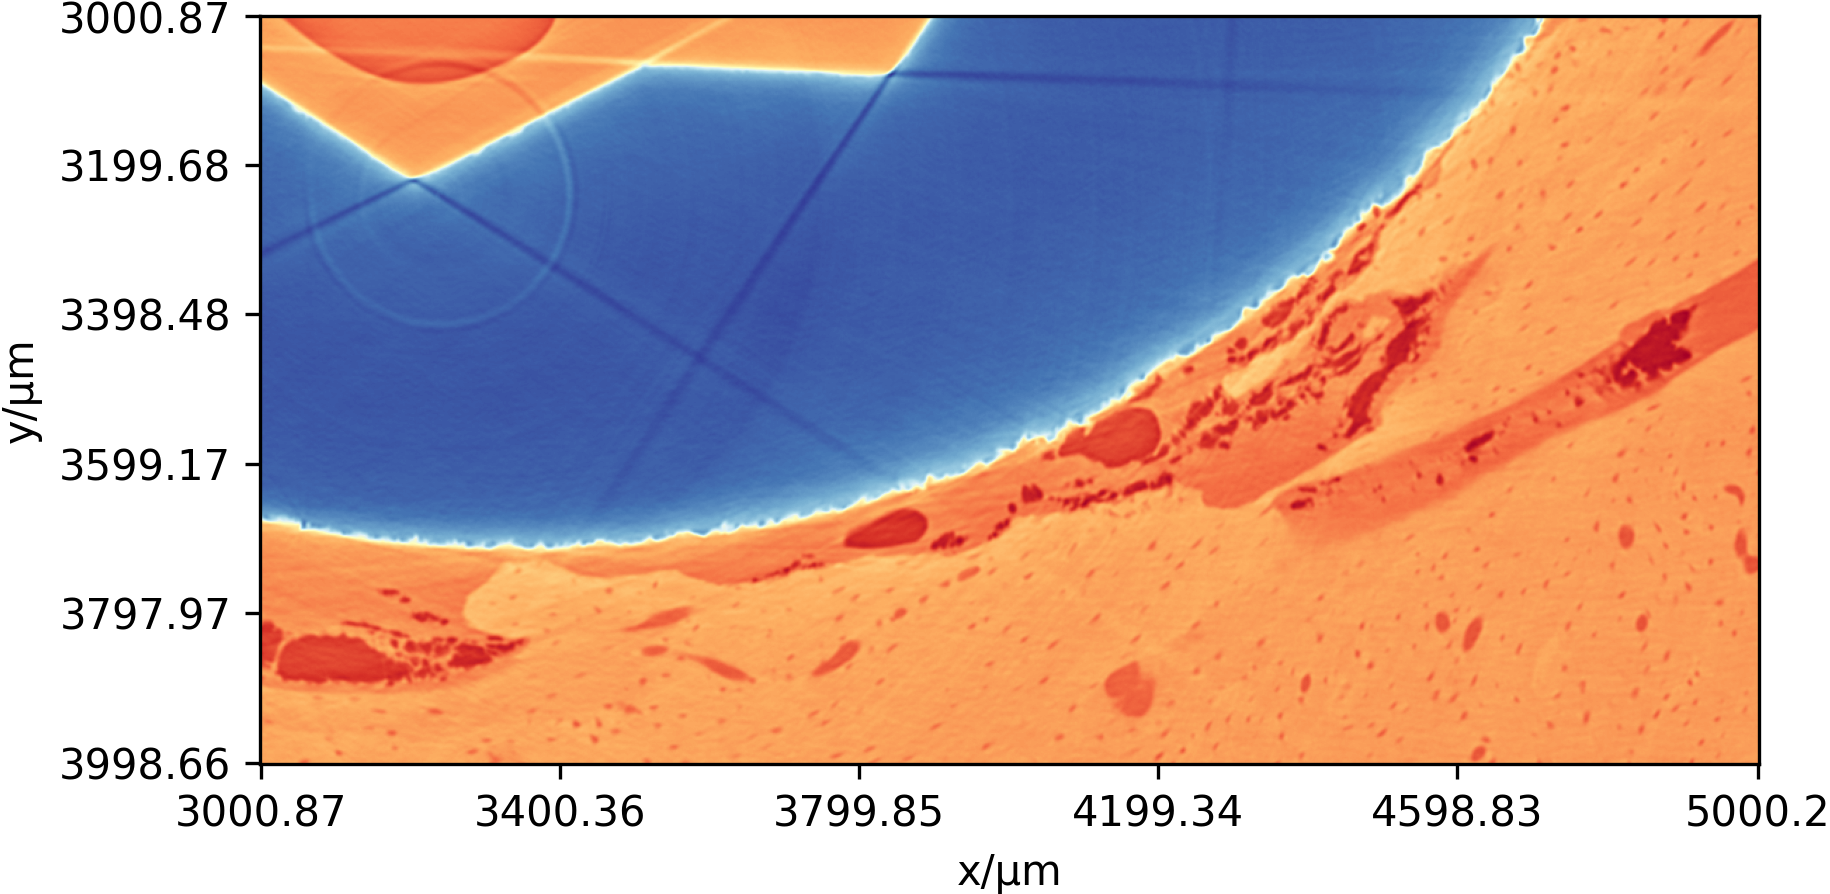
\includegraphics[width=\textwidth]{figures/770c_pag-bic-xy-1x.png}
\caption{Here we see a 1mm x 2mm region of an unscaled image slice in the XY dimension. It highlights
some of the imperfections and noise present in the data. We especially see artifacts within and
around the titanium implant. \aleksandar{Make label ticks smaller. Preferably same size as regular
text.}}
\label{fig:xy-slice}
\end{figure*}

In \cref{fig:xy-slice} and \cref{fig:yz-slice} we see zoomed in regions of the XY and YZ planes
of the same sample as shown in \cref{fig:3viewsample}.

\begin{figure}
\centering
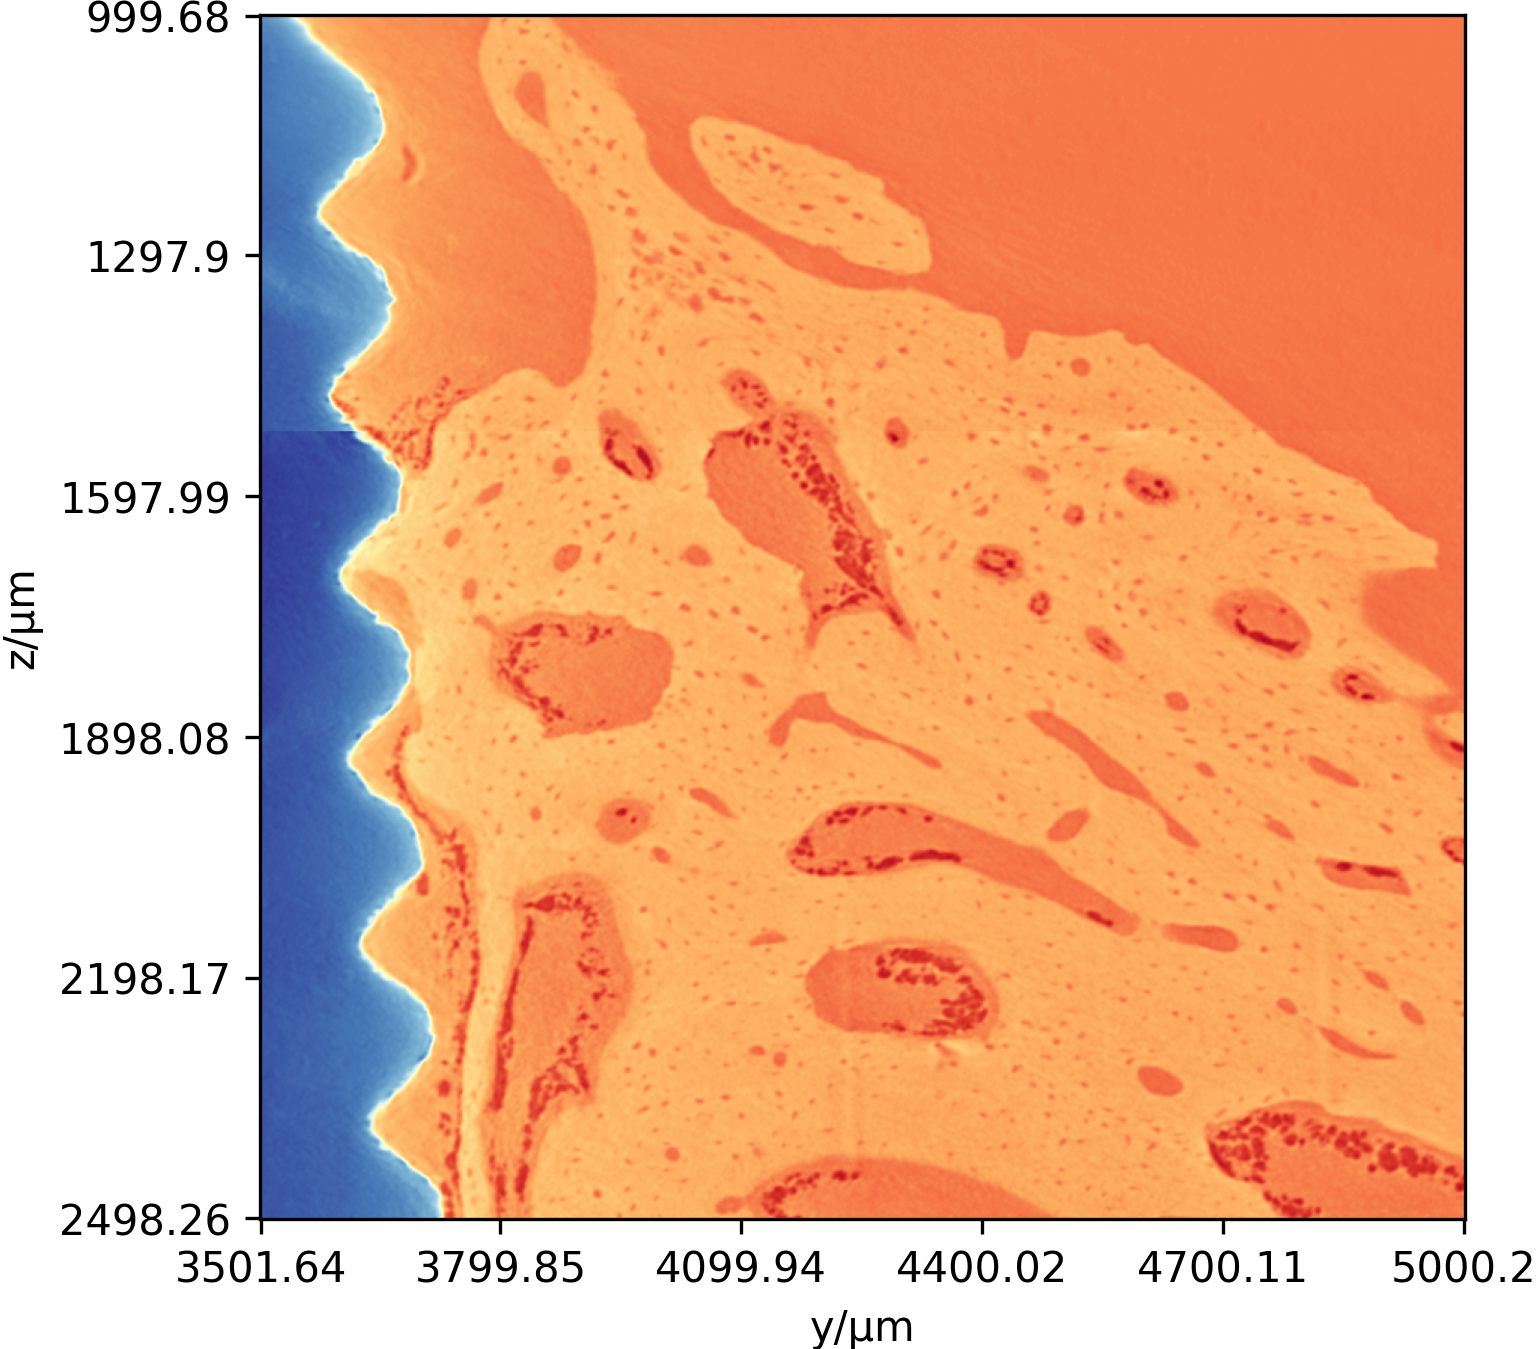
\includegraphics[width=\columnwidth]{figures/770c_pag-bic-yz-1x.png}
\caption{Here we see a 1.5mm x 1.5mm region of an unscaled image slice in the YZ dimension. This
hightlights noise and voxexl effects around the newly formed bone in the micro threaded part of
the titanium implant.}
\label{fig:yz-slice}
\end{figure}

Both planes display a broad selection of the various type of noise sources found in the data.

\subsection{Ring artifacts}

Looking at the XY-slice in \cref{fig:xy-slice} we see clear concentric ring artifacts emanating from
the center of the sample. Compared to the other artifacts mentioned, this effect is arising from
imperfections in the scanner setup. It can be from an uncalibrated or defect detector element. For
synchrotron radiation sources it can also occur from shifts and vibrations in the monochromator
crystal \citep{ringartifacts}.

\subsection{Projection artifacts}

Bright streaks with strong edges are seen from the sharp corners of the titanium implant. When
doing back projection, the \suggestion{carl}{symmetrybreaking}{symmetry breaking} is seen as smeared lines across the sample. This
can occur from the high pass filter used during filtered back projection, which exaggerates the
differences between adjacent elements \citep{ctnoise}.

\subsubsection{Beam hardening}

Medical CT and $\mu$CT both utilize poly-energetic beams, which can cause artifacts around high
density regions. This effect is called beam-hardening \aleksandar{ref}, and occurs when rays with
lower energy are attenuated more frequently, thus shifting the remaining photons to a higher
effective average photon energy. This offsets the local contrast, by overestimating
the attenuation, leaving lighter spots on the image. Many types of artifacts will typically be
present in these setups, but most are taken into account by calibration using phantoms and
pre-hardening the beam before it reaches the sample. Pre-hardening of the beam is done using
filters that attenuate the softest rays. Due to its common usage, much correction software exists
to account for noise and smaller imperfections during reconstruction \aleksandar{ref}.

Despite the practially mono-energetic rays from SR$\mu$CT, the source initially generates a
polychromatic spectrum. During monochromatisation this spectrum can still contain corrupted harmonic
components \citep{srnoise}. This leads to two distinct effects typically seen from beam-hardening.
\carl{Should be emphasized more. \textbackslash ref\{initial-beam-claim\} claims that there are no beam-hardening effects, and I think this reads as "well, yes, but no"}

\subsubsection{Dark and bright streaks}

Streaking artifacts occur at the dense implant region, but also in the transition from bone to softer
tissue. This effect is mostly seen in regions of large heterogeneity. When X-ray beams pass at angles
containing multiple dense obstacles, the beam is hardened more. Then for angles with fewer dense
obstacles the energy spectrum is preserved better. This produced the dark and bright streaks seen in
\cref{fig:xy-slice}.

For a hardened beam, softer x-rays are absorbed instead of successfully penetrating the object,
and will not contribute to image formation. High density structures such as the titanium implant
break the isotropy, making the projected X-ray mean energy spectrum dependent on incident orientation
\citep{srnoise}.

\subsubsection{Cupping effect}

A common artefact that occurs when beams pass more homogeneous cylindrical objects. Since beams
passing the middle will traverse more material compared to the edges, the beam is hardened more
towards the center and intensity becomes lower as a result. This can manifest itself in what
errnoeously looks to be dense peripheral regions at the edges.

\subsubsection{Compton scattering}

Lower energy rays contribute mostly with noise from scattering effects. A ray will propagate through a
material, get scattered and diffract from its initial trajectory. This gives a misrepresentation of
the attenuation along its initial trajectory. The artefacts seen from scattering are similar in
nature to those formed by beam hardening. This is because both effectively reduce the measured
attenuation. For energy levels of above 50KeV relevant for the data presented here, Compton
scattering is the dominating type \citep{compton}. The scattering occurs due to photon-electron
interaction between X-ray beam and the material it passes through. Like beam-hardening, scattering
will cause dark streaks across the image, where attenuation was highest.

\subsection{Other}

\aleksandar{Do we want to include: Undersampling and Poisson noise? Fringes at the edges of the
titanium implant due to phase-contrast effects (see srnoise ref), Partial volume artifacts which
are dependent on the voxel size and are mentioned briefly by Neldam et al., Refraction noise? All
effects seem to be handled already...}

For SR$\mu$CT a high photon flux allows for very short exposure times \citep{srexptime}.
This can help counter noise from suboptimal counting statistics\citep{srnoise}.
This is for example the case for Poisson noise.

\carl{Maybe a subsection describing how the old paper falls short close to the implant? I'm sure it'll be in the introduction as well, but shouldn't it also be explained in detail here? Maybe just a more detailed walkthrough of how they did it, and why it didn't work?}
\carl{Point to how the implant and bone/tissue masks are made in the "second" paper?}